%        File: kaiti.tex
%     Created: Tue Mar 12 06:00 PM 2013 C
% Last Change: Tue Mar 12 06:00 PM 2013 C
%xelatex
\documentclass[a4paper]{article}

\XeTeXlinebreaklocale "zh"
\XeTeXlinebreakskip = 0pt plus 1pt
\usepackage[cm-default]{fontspec}
\usepackage{xunicode,xltxtra}
\usepackage{indentfirst}
\usepackage{xeCJK}
\usepackage{graphicx}
\usepackage{algorithm}
\usepackage{algpseudocode}
\usepackage{amsmath}
\usepackage{xcolor}
\usepackage{listings}
\usepackage{fancyvrb}
\usepackage{tabularx}

\setCJKmainfont[BoldFont=STHeiti]{SimSun}
\setsansfont[Mapping=tex-text]{STHeiti} 
\setmainfont[BoldFont=STHeiti,ItalicFont=STKaiti]{SimSun} 

\begin{document}
\title{ 基于GIT的分布式实时编译及BUG分析系统}
\author{陈宇恒}
\maketitle
\date


\section{Linux开发流程与Git}

\section{0day的bug部分的设计实现的分析}
0day系统是由Linux核心开发者之一吴峰光最初开发的一套专门针对Linux内核代码质量控制的系统。
设计此系统有如下目的:
\begin{enumerate}
\item 
针对基于GIT的大规模多人同时开发软件,实现实时编译测试,在一天之内对出现问题的
代码提交做出响应并通知对应开发者;

\item
对成功编译的版本,进行运行测试。对于Linux内核,此测试通过KVM运行编译出来的内核镜像,
捕捉启动过程和若干测试程序导致的Kernel Panic,进行分析并通知开发者;

\item
捕捉代码修改对软件性能的影响。

\end{enumerate}


\subsection{0day系统组成}
本0day测试系统可以部署在广域网的多个集群上,各个集群之间只共享少量信息。先介绍单个集群的基本组成。

	\subsubsection{单集群系统主要组成}
	单个测试服务器集群由一个局域网中的多台服务器组成,各台服务器可以有较大的差距,0day测试系统
	可以根据不同机器的性能分配任务。每个集群中有一台特殊的服务器作为主节点,此节点担任一下角色:
	\begin{itemize}
		\item GIT镜像服务器,因为安全考虑,集群中只有此节点可以访问广域网。
		此节点定时从https://git.kernel.org/cgit/以轮训方式下载新的Linux Kernel 代码提交。其他节点
		从此服务器上通过GIT协议下载新Commit。
		\item NFS服务器。用于存放集群内共享的数据,例如编译结果、系统日志等。
		\item KVM测试调度器。此服务器上通过Apache Server上的一个CGI脚本,为KVM测试节点分配测试任务。
	\end{itemize}

	另外,集群中的每个节点又可以担任(或同时担任)一下角色:
	\begin{itemize}
	\item 编译服务器,用于编译不同Linux代码树的不同Commit
	\item KVM启动测试服务器,一台物理机上跑多个KVM,做内核启动测试,捕捉Kernel Panic
	\item LKP性能测试服务器,此服务器可能为真机或KVM虚拟机
	\end{itemize}

	\subsubsection{多集群系统组成}
	\begin{itemize}
		\item 如上一小节所示的$n$个独立测试集群,之间通过广域网连接
		\item 一个中心的Key-Value数据库,我们使用GIT设计了一个分布式的Key-Value
			数据库以实现集群间数据同步的功能。
	\end{itemize}

\subsection{各子系统实现}
\subsubsection{GIT镜像服务器}
	在Linux开发过程中,各个子系统开发者都维护着自己的开发代码树,测试通过后再向Linus维护的
	主代码树linux提交代码。这些代码树的列表可以在https://git.kernel.org/cgit/上获得。GIT镜像服务器更新的主逻辑如下:
	\begin{Verbatim}[frame=single]
	for repo in  ALL_REPOS
		git fetch –no-tags
			if updated
				update-commit-list
	\end{Verbatim}
	这里commit-list记录了这个repo的HEAD到最近一次从upstream分支分叉之间的所有commit。这个文件将作为编译服务器的输入。

\subsubsection{KVM调度器}
	这个子系统实际上是一个HTTP Server,当接受到客户端(KVM测试服务器)的请求时,调度器的CGI脚本检查查找
	还没有运行测试过的内核镜像,返回服务器端。另外,此子系统还支持bisect运行时错误。关于bisect的具体方法见下面。

\subsubsection{基于GIT的多集群Key-Value数据库}  
见下面

\subsubsection{编译服务器kernel-build逻辑}
	此子系统是0day编译测试的核心,在实际部署中,每个服务器运行多个kernel-build进程,每个进程与其他编译进程
	需要共享的唯一信息是一个Error ID  Key-Value数据库,除此之外完全独立。由于编译进程良好的独立性,非常有利于大规模多机器部署。
	编译服务器实现如下功能:
	\begin{enumerate}
		\item 通过GIT镜像服务器更新本进程对应的本机内核代码树镜像
		\item
			通过commit-list找到新的commit,若有多个tree有更新,可能先merge,减少编译量
		\item 使用预先分配的(architecture, configuration)
			配置对新的HEAD进行编译,将编译出多个不同体系结构、配置的内核
		\item 编译同时调用静态代码检查工具做检查
		\item 若编译错误或警告,进行Bisect
		\item 安装内核到NFS,准备Boot测试
	\end{enumerate}
	由上述过程,可知不同进程的任务划分是通过(architecture,
	configuration)对完成的。


	\begin{Verbatim}[frame=single]
	acquire_build_error_id_repo
	compile_test
		reset_upstream
		while true
			compile_archs
			for remote in commit-list
				if has new commit
					git remote update
		end
				
	\end{Verbatim}

	\begin{Verbatim}[frame=single]
	compile_archs
		foreach ARCH
			generate randconfigs
			merge_updated_branches
			foreach updated_branch
				foreach commit_list
					foreach config
						compile_one_config
			compile_queue_tasks
	\end{Verbatim}

	内核编译是一个复杂的过程,但是考虑到两个相邻的Commit之间变化应该不会太大,利用这种局部性,我们可以使用一些优化手段减少编译时间,
	做到每个Patch被提交之后1天内能被测试到。0day系统使用到的加速方法如下:
	\begin{enumerate}
		\item 使用tmpfs存放目标文件
		\item 充分利用Kernel Build
			System的特性,非必要时只编译单个文件或模块,这在对单个文件的Error或Warning
			做Bisect时有很大作用
		\item 使用CCache
	\end{enumerate}

	另外,0day系统的一个重要功能是错误的筛选和去重复。这个功能可以解决编译器和代码检查工具输出大量
	重复或无效信息的问题,为开发者提供一个清晰的Bug报告。本功能在Error
	ID一节介绍

\subsubsection{Boot测试服务器逻辑}

	XXXXX

%%%%%%%%%%%%%%%%%%%%%%%%%%%
\section{相关工作}

\subsection{Fast 2013 Best Paper}
\emph{A Study of Linux File System Evolution}\\

本文主要通过Linux开发过程中Git Commit中开发者给出的patch信息,分析
Linux Kernel文件子系统的代码演化。通过分析8年来Linux文件系统相关的
5079个patch,提出了一些新颖且令人惊讶的现象。这些对Patch分析的结果
非常有利于以后的文件系统开发和相关Bug自动分析工具的开发。

Git中的一个Patch如下图\ref{fig:patch}所示:
\begin{figure}[h]
	\begin{center}
		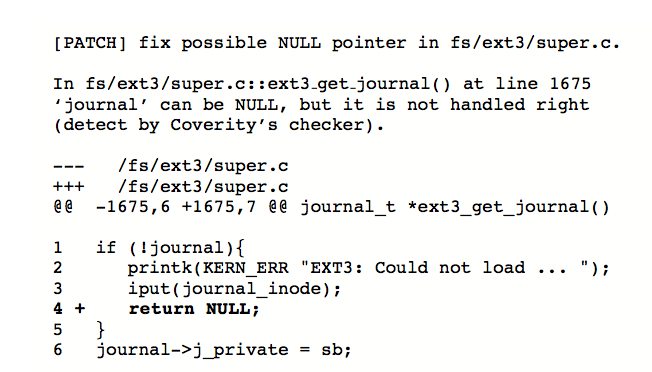
\includegraphics[width=0.8\textwidth]{patch.png}
	\end{center}
	\caption{Patch实例}
	\label{fig:patch}
\end{figure}

文章把Patch做了如表\ref{tab:patch_clas}的分类。

\begin{table}[h]
	\centering
	\begin{tabular}{c| p{5cm} }
		类型 &  描述 \\
		\hline
		Bug  &  Bug修复 \\
		\hline
		性能 &  改进设计、提高文件系统性能(如减少锁的使用)\\
		\hline
		可靠性 &   提升文件系统可靠性(如加入数据检验)\\
		\hline
		新特性 &  引入新特性 \\
		\hline
		维护  &  简单的代码维护,例如改进API \\

	\end{tabular}
	\caption{Patch分类}
	\label{tab:patch_clas}
\end{table}


本文作者手工查看、分析、归类了Ext3/Ext4/XFS/Btrfs/ReiserFS/JFS这
几个文件系统相关的5079个patch,仔细整理分析后回答了例如“最多的patch
是那个方面的patch?”和“最常见的文件系统Bug是什么?”。

作者发现,在这5000多个Patch中,一般维护性的patch占了一半。接着有
40\%的Patch是bug修复,这是本文关心的部分。作者在文中对这些Bug修复
的Patch做了详尽的统计分析,揭示的文件系统Bug分布的规律。

对于文件系统的Bug,作者总结了如下的一些规律

\begin{enumerate}
	\item XXX
\end{enumerate}



\subsection{Yuanyuan Zhou  OSDI 2012}
\emph{Be Conservative: Enhancing Failure Diagnosis with Proactive Logging}

这一论文更偏重与运行时错误的分析。

\subsubsection{摘要}
软件系统在实际运行中出错时,软件日志中的错误和警告信息经常是唯一可以用于分析定位
底层错误的手段。因此,这些Log的有效性就具有很强的重要性。但是,很少有人研究现有
日志信息的搜集方法和如何提高这些日志的有效性。本文针对五个广泛使用的大型开源软件做了
研究。从250个随机采样的系统错误中,发现有大半错误无法通过现有的日志信息很好地诊断
出来。但是另一方面,进一步分析显示,大多数这些错误可以分为几个常见的错误模式(例如
系统调用返回错误)。如果对这些错误模式进行适当的日志记录,可以极大地方便诊断错误和
调试。进一步,本文提出了一个Errlog自动日志输出添加工具。此工具自动在出现可能错误前
代码位置上添加日志输出信息。用户使用反馈显示,在只带来1.4\%性能损失的同时,减少60.7\%
的错误诊断时间。


%%%%%%%%%%%%%%%%%%%%%%%%%

\section{基于Git的Error ID数据库实现}
为了避免重复向开发者报告同一问题,0day系统使用一个广域网上同步的Error
ID数据库用来判断一个新的错误是否出现过。此数据库本质是一个Key-Value哈希表。
为了避免单独维护这一数据库服务器,我们采用GIT实现了这一功能。此实现可以保证
并发访问的正确性。

此全局Error ID数据库需要支持客户端执行操作:
\begin{enumerate}
	\item 查询一个Key是否存在
	\item 若Key不存在,添加一个(Key,Value)记录
\end{enumerate}

数据一致性要求:

\begin{enumerate}
	\item 查询操作可以看到所有已经成功添加到主节点的记录
	\item 若一个记录已经成功添加到主节点,则不能被重新添加,
		否则更新应该成功
\end{enumerate}

由于我们使用Git实现支持以上功能的数据库,这意味这个数据库在整个广域网上有多个
分布式的副本。为了保持同步,我们使用了Github服务器作为主节点,每个集群作为
子节点使用以下算法保证查询和更新操作遵守数据的一致性要求。

\begin{Verbatim}[frame=single]
	test_set(keys,values)
	{
		for k,v in keys,values
			if k exists
				continue
			write v to file k
			git add k
		done
	}
\end{Verbatim}

\begin{Verbatim}[frame=single]
	while
		git pull --ff-only || {
			#should not error, try reset
			git reset --hard HEAD^
			continue
		}

		test_set keys,values

		git commit -a

		#if push success, finish
		git push && break

		#push failed, remote centeral repo updated
		git reset --hard HEAD^

	done
\end{Verbatim}

以上算法解决了广域网上各个集群上的同步问题。由于以上算法对Git的操作不是原子的,
多个本地进程同时对一个本地Git Repo操作会出现问题。考虑到这个数据库大小不会
很大,我们使用多份拷贝的方式解决此问题。若系统中有N个数据库客户端进程在运行,则
在内存中保存N份Repo的拷贝,每个客户端进程绑定到各自的Repo上。这种设置不会影响
算法的正确性。

由于集群防火墙安全设置,每个集群中除了一个出口节点外,其他机器均无法连接
广域网,因此实际实现时,每个客户端执行以上算法时,均push到出口节点上的镜像,
由镜像上的Git Hook转发Push请求转发到远程服务器,并把错误逐层返回。


\end{document}


